% =====================================================================================
% final_report_WaleedAhmed_ICLR2026.tex
% Formatted according to the ICLR 2026 conference author guidelines
% (iclr2026_conference.sty / .bst). Compile with pdfLaTeX; run twice for references.
% =====================================================================================
\documentclass{article}

\usepackage{iclr2026_conference,times}
\input{math_commands.tex}

\usepackage{hyperref}
\usepackage{url}
\usepackage{graphicx}
\graphicspath{{figures/}}
\usepackage{booktabs}
\usepackage{multirow}
\usepackage{amsmath}
\usepackage{amssymb}

\hypersetup{pdftitle={final_report_WaleedAhmed_ICLR2026 (ICLR 2026 format)},
            pdfauthor={Waleed Ahmed}}

\title{
When Does an Explicit Homophily Prior Help? \\
Markov Random Fields, Variational Inference and MCMC \\
for Low-Label Node Classification
}

\author{Waleed Ahmed\thanks{Report formatted according to the ICLR 2026 conference
author guidelines (\texttt{iclr2026\_conference.sty}).} \\
School of Computing Science \\
Simon Fraser University \\
\texttt{waa18@sfu.ca}
}

\iclrfinalcopy

\begin{document}

\maketitle

\begin{abstract}
Graph neural networks are justified by a \emph{homophily} assumption -- nodes joined by an edge
tend to share a label -- but the assumption is buried inside the architecture, so its
contribution is never measured on its own. We take the assumption out of the architecture, write
it down as an explicit pairwise Markov random field (MRF) over the labels, and measure under
controlled conditions when stating it explicitly helps. We compare a Laplacian smoothness
penalty on the training loss, an expected rule-violation penalty, and a Potts MRF whose unary
potentials are a frozen network's logits and whose posterior we compute with mean-field
variational inference, loopy belief propagation, and Gibbs sampling -- all validated against
exact marginals from variable elimination (7{,}744 model runs; 11{,}280 exact-inference
comparisons; protocol fixed in advance). Our pre-registered hypothesis that the prior helps most
when labels are scarcest is \emph{refuted and reversed}: the benefit grows with supervision
($-7.07$ accuracy points, 95\% CI $[-10.26,-3.91]$), because an MRF propagates label information
rather than creating it. On synthetic graphs where the assumption's truth is controlled, a prior
whose strength is fixed in advance loses up to 45 points through posterior collapse, while the
same prior tuned on validation data never loses more than 0.5. Finally, a degree-preserving
rewiring control shows the popular Laplacian penalty keeps most of its benefit on a graph with
no label structure at all: it acts largely as a generic regularizer, not as relational
reasoning.
\end{abstract}

\section{Introduction and research problem}

Many prediction problems are relational: the objects being classified are connected, and the
connections carry information. Citation networks are the canonical example -- a paper's topic is
predictable from the topics of the papers it cites. Graph neural networks (GNNs) exploit this by
smoothing representations along edges, and the assumption that justifies the smoothing is
\emph{homophily}: an edge is evidence that its endpoints share a label. The regime where this
should matter most is \emph{low-label} classification, where only a handful of nodes per class
are annotated and prior knowledge must substitute for missing supervision.

\paragraph{Problem statement.} The computational problem is transductive node classification.
\emph{Input:} a graph $G=(V,E)$ with $n=|V|$ nodes, a feature matrix $X\in\R^{n\times d}$, and
labels $y_i\in\{1,\dots,C\}$ observed on a small training set (we study $m\in\{1,2,5,10,20\}$
labeled nodes per class) together with a validation set used only for model selection.
\emph{Output:} a predicted label -- and, for probabilistic models, a posterior marginal
$q_i(c)\approx p(y_i{=}c\mid X,G)$ -- for every unlabeled node, evaluated on a held-out test
set. \emph{Assumptions:} the setting is transductive (features and edges of all nodes are
visible during training; only labels are hidden); the candidate prior is pairwise homophily; and
the classifier backbone is held fixed so that only the treatment of the prior varies.

\paragraph{Why existing practice is not satisfactory.} Two gaps motivate this study. First, the
value of the homophily assumption is almost never measured, because it is not separable from the
architecture that embodies it: a graph convolution is provably a form of Laplacian smoothing
\citep{li2018deeper}, so adding a homophily-flavoured penalty to a GCN -- the design in our own
project proposal -- asks ``does more of the same help?'' rather than ``does the prior help?''.
Second, when the assumption \emph{is} written down explicitly, it is usually as a heuristic
penalty on network outputs described in probabilistic language; no random field is actually
defined, no posterior is computed, and consequently nothing can be said about when the
assumption is false or what happens then. Existing benchmark practice compounds the problem:
real datasets have fixed homophily, so the failure regime of the prior cannot be observed on
them at all.

\paragraph{What we do.} We hold one backbone fixed (a two-layer GCN, and a graph-blind MLP as
the clean control) and impose the \emph{same} assumption three ways of increasing probabilistic
seriousness: a Laplacian penalty at training time, an expected rule-violation penalty at
training time, and an explicit Potts MRF over the labels at inference time, solved with
mean-field variational inference and audited with belief propagation, Gibbs sampling, and exact
inference. We evaluate under a protocol fixed before any experiment ran, crossing label scarcity
with a synthetic environment in which the truth of the assumption is dialed from $5\%$ to
$90\%$ edge homophily at constant degree. Three findings emerge: the prior's value tracks the
quality of the evidence it propagates rather than label scarcity (our pre-registered hypothesis
was refuted in the opposite direction); misspecification harms only a prior that is committed to
in advance; and the widely used Laplacian penalty fails a causal control that the MRF passes,
revealing it to be largely a generic regularizer.

\section{Related work}

\paragraph{Graph-based semi-supervised learning first formalized homophily as a probabilistic
model.} \citet{zhu2003semi} modeled labels as a random field over the graph, clamped the
observed labels as evidence, and inferred the rest by propagation; label propagation and its
descendants remain strong low-label baselines. Our MRF is this idea with learned unary
potentials, and label propagation is one of our baselines. The difference is the question: prior
work asks \emph{whether} the field helps on homophilous benchmarks; we ask \emph{when} it helps,
by manipulating the truth of the assumption directly.

\paragraph{GNNs internalize the same assumption in the architecture.} The GCN of
\citet{kipf2017semi} averages representations over neighborhoods, which \citet{li2018deeper}
identified as Laplacian smoothing with oversmoothing as its failure mode. A line of work has
mapped where this implicit assumption breaks: heterophilous graphs \citep{zhu2020beyond},
the observation that low homophily need not mean an uninformative graph \citep{ma2022homophily},
and better homophily measures \citep{platonov2023characterizing}. We differ in that we measure
the \emph{marginal} value of making the assumption explicit on top of (and separately from) the
architecture that already contains it -- a comparison the cited work does not run.

\paragraph{Neural-symbolic methods impose rules as differentiable penalties.} Logic rules have
been distilled into network weights \citep{hu2016harnessing}, and the semantic loss of
\citet{xu2018semantic} penalizes the probability that a constraint is violated under the model's
own distribution; our rule-violation penalty is exactly this construction for the rule
$\textsc{Edge}(i,j)\Rightarrow\textsc{SameClass}(i,j)$. These works propose mechanisms and
report gains; none tests whether the penalty's benefit actually flows through the relations the
rule mentions. Our degree-preserving rewiring control is precisely that test, and the popular
Laplacian variant fails it.

\paragraph{Hybrid models combine GNNs with random fields, or correct predictions post hoc.}
GMNN \citep{qu2019gmnn} trains a GNN--CRF hybrid with variational EM; APPNP
\citep{gasteiger2019predict} and Correct \& Smooth \citep{huang2021combining} decouple
prediction from propagation and show post-hoc correction of a simple predictor is highly
effective -- the design our inference-time MRF follows. These papers propose models and
demonstrate accuracy; we hold the model class fixed, pre-register hypotheses, and characterize
the conditions (label budget, homophily level, commitment to the prior) under which the shared
idea pays, with the inference itself validated rather than assumed correct.

\paragraph{Approximate inference has been benchmarked against exact answers before, and
evaluation pitfalls in GNN research are documented.} \citet{murphy1999loopy} scored loopy belief
propagation against exact marginals on tractable networks; we adopt that methodology as a
\emph{validation layer} for all three of our inference engines, with the chromatic Gibbs
schedule of \citet{gonzalez2011parallel}. \citet{shchur2018pitfalls} showed single-split GNN
evaluation is unreliable, which motivates our paired multi-seed protocol; our synthetic
generator is the contextual stochastic block model of \citet{deshpande2018contextual}.

\section{Approach}

\subsection{Research hypotheses}

The study was pre-registered: hypotheses, comparisons, grids, seeds, and the analysis plan were
version-controlled before any experiment ran. The confirmatory hypotheses are:

\begin{itemize}\itemsep2pt
\item \textbf{H1 (scarcity).} The benefit of the explicit prior is largest when labels are
scarcest: the paired advantage of the MRF over its own unary model is larger at $m{=}2$ than at
$m{=}20$ labels per class.
\item \textbf{H2a (benefit tracks truth).} With the prior's strength fixed in advance, its
benefit is larger at edge homophily $h{=}0.9$ than at $h{=}0.5$.
\item \textbf{H2b (misspecification harms).} With the prior's strength fixed in advance, the
prior \emph{reduces} accuracy at $h{=}0.05$.
\end{itemize}

A methodological requirement underlies all three: conclusions must be attributable to the
\emph{model}, not to the approximate inference used to fit it, which we enforce by validating
every inference routine against exact marginals.

\subsection{One assumption, three impositions}

Let $s_i(c)$ be the logits of a trained encoder (MLP or GCN) and
$p_i=\mathrm{softmax}(s_i)$. The homophily assumption enters in three ways
(Figure~\ref{fig:schematic}).

\textbf{(M2) Laplacian penalty} -- the model from our proposal -- penalizes disagreement across
edges during training, with $\lambda$ acting as a prior precision in a MAP reading:
\begin{equation}
\mathcal{L}_{\rm lap}=\frac{1}{|E|}\sum_{(i,j)\in E}\|p_i-p_j\|_2^2,\qquad
\mathcal{L}=\mathcal{L}_{\rm CE}+\lambda\,\mathcal{L}_{\rm lap}.
\end{equation}

\textbf{(M3) Expected rule violation.} Treating predictions as independent label distributions,
$\Pr(y_i{=}y_j)=p_i^\top p_j$, so the probability that the rule is violated yields a semantic
loss \citep{xu2018semantic}:
$\mathcal{L}_{\rm rule}=\frac{1}{|E|}\sum_{(i,j)\in E}(1-p_i^\top p_j)$.

\textbf{(M4) Explicit Potts MRF.} Rather than nudging outputs, we define a distribution over
the labels themselves, with the \emph{frozen} logits as unary potentials:
\begin{equation}
p(y\mid X,G)\;\propto\;\exp\Big[\textstyle\sum_{i\in V} s_i(y_i)
\;+\;\beta\sum_{(i,j)\in E}\mathbf{1}[y_i=y_j]\Big],
\label{eq:potts}
\end{equation}
where $\beta\ge0$ encodes belief in the assumption and $\beta=0$ recovers the plain network
exactly (a correctness test). Prediction computes posterior marginals and takes the argmax.
Freezing the logits is what makes the comparison clean: every MRF variant consumes identical
evidence, so differences are caused by the prior and the inference, not by a differently fitted
network.

\begin{figure}[t]
\begin{center}
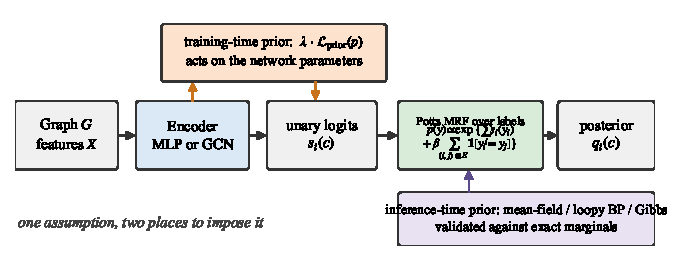
\includegraphics[width=\linewidth]{fig1_schematic.pdf}
\end{center}
\caption{One assumption, two places to impose it. Upper path: a penalty on the training loss
changes the network's parameters. Lower path: the trained network's logits become unary
potentials of a Potts MRF whose posterior is recomputed at test time with the network frozen;
every inference routine is validated against exact marginals first.}
\label{fig:schematic}
\end{figure}

\paragraph{Proposition 1 (shared statistic).} With edgewise agreement
$A(p)=\sum_{(i,j)\in E}p_i^\top p_j$:
\begin{align}
\mathcal{L}_{\rm rule}&=1-\tfrac{1}{|E|}A(p),\qquad
\mathcal{L}_{\rm lap}=\tfrac{1}{|E|}\textstyle\sum_{(i,j)\in E}\big(\|p_i\|^2+\|p_j\|^2\big)
-\tfrac{2}{|E|}A(p),\\
\mathcal{F}_{\rm MF}(q)&=\textstyle\sum_i q_i^\top s_i+\beta A(q)+\sum_i H(q_i).
\end{align}
\emph{Proof:} expand $\|p_i-p_j\|^2$ and sum; $\mathcal{F}_{\rm MF}$ is the evidence lower
bound for Eq.~\ref{eq:potts} under $q(y)=\prod_i q_i(y_i)$. $\square$\;
All three objectives are driven by the same pairwise statistic $A$ but differ in what is
optimized (parameters during training vs.\ the posterior at test time) and in the companion
term: the Laplacian form carries an extra $\sum_i\deg_i\|p_i\|^2$, a \emph{confidence penalty}
that acts regardless of what the graph says, while the variational objective carries entropy.
This proposition generates the falsifiable prediction tested by our rewiring control.

\subsection{Computing the posterior}

Exact marginals of Eq.~\ref{eq:potts} are intractable at scale ($7^{2708}$ configurations on
Cora), so we implemented three approximate algorithms and an exact reference.

\textbf{Mean-field variational inference} (primary engine) maximizes the ELBO over a fully
factorized family by coordinate ascent,
\begin{equation}
q_i(c)\;\propto\;\exp\Big[s_i(c)+\beta\textstyle\sum_{j\in N(i)}q_j(c)\Big],
\label{eq:mf}
\end{equation}
updating one \emph{graph-color class} at a time: same-color nodes share no edge, so a whole
class updates simultaneously while remaining exact block coordinate ascent -- vectorized and
provably ELBO-monotone, which we assert at runtime. We always run to convergence; the iteration
count is never a tuned hyperparameter, since a half-converged approximation would confound
``the model is worse'' with ``we stopped early''.

\textbf{Loopy belief propagation} is exact on trees (a strong correctness test) and approximate
on cyclic graphs; we use damped updates and exploit the Potts structure for $O(C)$ rather than
$O(C^2)$ messages. \textbf{Gibbs sampling} resamples an entire color class at once, valid
because same-color nodes are conditionally independent \citep{gonzalez2011parallel}; we use the
Rao-Blackwellized estimator (averaging conditional probability vectors rather than counting
states) and monitor split $\hat{R}$ and effective sample size, refusing to trust runs that fail
these diagnostics. \textbf{Exact inference} computes true marginals two independent ways --
brute-force enumeration when $C^n\le 5{\times}10^6$ and repeated variable elimination with a
min-fill ordering otherwise -- required to agree to $10^{-10}$ before use as ground truth.

\subsection{A synthetic environment where the assumption's truth is controlled}

Real graphs have fixed homophily, so we generate contextual stochastic block models
\citep{deshpande2018contextual}: $n=2800$ nodes in $C=7$ equal classes, edge probabilities
$p_{\rm in}=hk/(n_c-1)$ within class and $p_{\rm out}=(1-h)k/(n-n_c)$ across, and features
$x_i\sim\mathcal{N}(\mu_{y_i},\sigma_x^2 I)$. This holds expected degree at $k=8$ for every
target homophily $h$, so degree cannot confound the sweep. Knowing the generator yields two
reference ceilings: the Bayes-optimal feature-only classifier (\textsc{Oracle-F}; nearest class
mean) and \textsc{Oracle-G}, which also uses the graph with the generator-implied coupling
$\beta_{\rm gen}=\log(p_{\rm in}/p_{\rm out})$. The noise $\sigma_x$ was fixed once on
quarantined pilot graphs by requiring \textsc{Oracle-F} accuracy in $[0.70,0.80]$, and never
retuned.

\paragraph{Two prior regimes.} If $\beta$ is selected on validation data then, because
$\beta=0$ nests the baseline, a wrong prior is tuned away and can never hurt -- so harm would be
unobservable by construction. We therefore evaluate both a \textbf{tuned} regime ($\beta$
selected per condition; the prior as an \emph{option}) and a \textbf{dogmatic} regime ($\beta$
fixed at the value selected on a highly homophilous reference graph and applied everywhere; the
prior as an \emph{assumption} committed to in advance).

\subsection{Implementation, correctness gates, and acknowledged code}

All models and all four inference engines were implemented by us in Python on top of open-source
libraries: PyTorch (CPU) for training; PyTorch Geometric for the \texttt{GCNConv} layer and the
Planetoid dataset loaders; NetworkX for greedy graph coloring; SciPy for statistical tests;
ArviZ for $\hat{R}$ and effective sample size; NumPy, pandas, and Matplotlib for analysis and
figures. No model or inference code was taken from prior work. Before any experiment, gate
tests had to pass: $\lambda{=}0$ reproduces the plain GCN to $<10^{-5}$; $\beta{=}0$ reproduces
$\mathrm{softmax}(s)$ to $2.1{\times}10^{-14}$ for every engine; enumeration and variable
elimination agree to $<10^{-10}$; BP matches exact marginals on trees; the ELBO never decreases;
and permuting test labels leaves training output bit-identical, proving test labels cannot leak
into training.

\section{Results}

\subsection{Experimental setup}

\paragraph{Datasets and baselines.} We use Cora and CiteSeer
\citep{sen2008collective,yang2016revisiting} in the standard Planetoid split, and the synthetic
generator of \S3.4 (Table~\ref{tab:data}); statistics are recomputed from the loaded data. The
points of comparison are: the MLP (features only), label propagation (graph and training labels
only), the GCN (both), the GCN with each training-time penalty, and the Potts MRF applied to the
MLP's and to the GCN's frozen logits. The MRF-on-MLP cell is the clean test of the explicit
prior -- there the graph enters \emph{only} through the MRF -- while MRF-on-GCN measures its
marginal value on top of the implicit architectural prior.

\begin{table}[t]
\caption{Dataset statistics, recomputed from the loaded data ($h_{\rm adj}$ = adjusted
homophily, LI = label informativeness). CSBM expected degree is 8.0 at every $h$ by
construction; at $h{=}0.05$ adjusted homophily is negative, i.e.\ the graph is heterophilous.}
\label{tab:data}
\begin{center}
\small
\begin{tabular}{lrrrrrrr}
\toprule
\textbf{Dataset} & \textbf{Nodes} & \textbf{Edges} & \textbf{Feat.} & \textbf{$C$} &
\textbf{Degree} & \textbf{$h_{\rm edge}$} & \textbf{$h_{\rm adj}$ / LI} \\
\midrule
Cora            & 2{,}708 & 5{,}278 & 1{,}433 & 7 & 3.90 & 0.810 & 0.771 / 0.590 \\
CiteSeer        & 3{,}327 & 4{,}552 & 3{,}703 & 6 & 2.74 & 0.736 & 0.671 / 0.451 \\
CSBM $h{=}0.05$ & 2{,}800 & $\approx$11.1k & 32 & 7 & 7.95 & 0.051 & $-0.107$ / 0.023 \\
CSBM $h{=}0.50$ & 2{,}800 & $\approx$11.2k & 32 & 7 & 7.98 & 0.499 & 0.416 / 0.183 \\
CSBM $h{=}0.90$ & 2{,}800 & $\approx$11.1k & 32 & 7 & 7.93 & 0.903 & 0.886 / 0.747 \\
\bottomrule
\end{tabular}
\end{center}
\end{table}

\paragraph{Protocol and statistics.} Label budgets $m\in\{1,2,5,10,20\}$ per class, stratified
and nested across $m$; 10 random seeds (30 on the confirmatory cells); backbone hyperparameters
tuned once per dataset and architecture at $m{=}5$, then frozen; prior strength tuned on
validation with an equal budget of six configurations per model; early stopping on validation
accuracy; model selection is a pure function of validation metrics and never reads a test
column. Every comparison is \emph{paired}: within a seed, all models share the split and the
trained checkpoint, and we report mean paired differences with 95\% BCa bootstrap intervals
($B{=}10{,}000$) and sign counts. Only H1, H2a, and H2b receive hypothesis tests
(Holm-corrected two-sided Wilcoxon signed-rank); all other comparisons are estimates labeled
exploratory. On real data, seeds vary the training sample and initialization on a fixed graph
and test set, so intervals describe run-to-run variability; only the synthetic experiment
redraws the graph per seed. Metrics: accuracy and macro-F1 (the two named in our proposal),
NLL, Brier score, and expected calibration error for distributional quality, plus rule
satisfaction $R=\frac{1}{|E|}\sum p_i^\top p_j$ and argmax edge agreement as prior diagnostics.
In total: 7{,}744 model runs and 11{,}280 exact-inference comparisons on CPU; 13 automated
audit checks pass.

\subsection{Evidence for the three hypotheses}

\paragraph{H1 -- refuted, with the effect reversed.} The pre-registered comparison asked
whether the MRF's advantage over the MLP is larger at $m{=}2$ than at $m{=}20$. Over 30 paired
seeds the difference-of-differences is $\theta=-7.07$ points, 95\% CI $[-10.26,-3.91]$,
$p=6.6{\times}10^{-4}$, with 7 of 30 seeds in the predicted direction. Under macro-F1 the
reversal is sharper still ($\theta=-9.73$, CI $[-13.10,-6.43]$, $p=8{\times}10^{-6}$).
Figure~\ref{fig:lowlabel} shows the full curves: against the GCN, the prior's benefit
\emph{shrinks} with supervision ($+4.38\to+0.59$ points from $m{=}1$ to $m{=}20$ for the
Laplacian penalty); against the MLP it \emph{grows} ($+4.45\to+19.55$). CiteSeer reproduces the
pattern ($+5.34$, $+12.46$, $+10.09$ points at $m=1,5,20$; 10 of 10 seeds each).
Table~\ref{tab:metrics} reports the full metric suite.

\begin{figure}[t]
\begin{center}
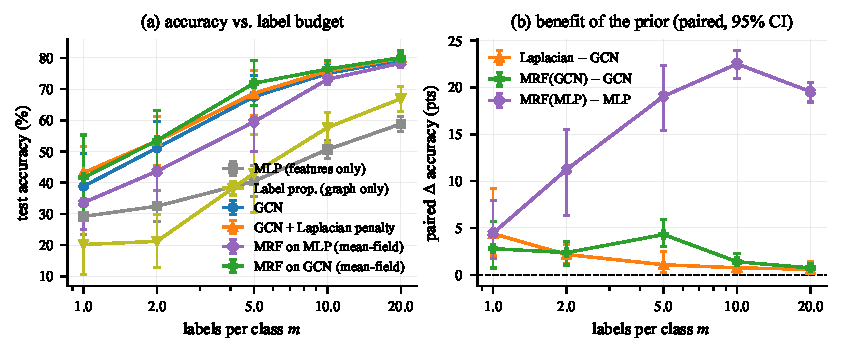
\includegraphics[width=0.95\linewidth]{fig2_low_label.pdf}
\end{center}
\caption{Cora, 10 paired seeds. (a) Test accuracy against labels per class ($\pm1$ s.d.).
(b) Paired differences with 95\% bootstrap intervals: the explicit prior's benefit over the GCN
decays with supervision while its benefit over the graph-blind MLP grows.}
\label{fig:lowlabel}
\end{figure}

\begin{table}[t]
\caption{Metric suite on Cora, mean over 10 paired seeds (exact values behind
Figure~\ref{fig:lowlabel}a). Macro-F1 tracks accuracy closely, so no conclusion depends on the
choice between them; the probability metrics (lower is better) separate the models differently
-- see \S\ref{sec:analysis}.}
\label{tab:metrics}
\begin{center}
\footnotesize
\begin{tabular}{lrrrrr@{\hskip 1.1em}rrrrr}
\toprule
& \multicolumn{5}{c}{\textbf{$m=5$ labels/class}} & \multicolumn{5}{c}{\textbf{$m=20$ labels/class}} \\
\cmidrule(lr){2-6}\cmidrule(lr){7-11}
\textbf{Model} & Acc & F1 & NLL & Brier & ECE & Acc & F1 & NLL & Brier & ECE \\
\midrule
MLP (features only)       & 40.5 & 39.4 & 1.727 & 0.778 & 0.148 & 58.9 & 57.3 & 1.362 & 0.623 & 0.196 \\
Label propagation         & 43.0 & 44.9 & 1.592 & 0.707 & 0.226 & 66.9 & 69.3 & 1.123 & 0.498 & 0.218 \\
GCN                       & 67.6 & 67.4 & 1.407 & 0.646 & 0.362 & 79.4 & 78.4 & 1.055 & 0.487 & 0.359 \\
\ + Laplacian penalty (M2) & 68.7 & 68.5 & 1.460 & 0.669 & 0.396 & 79.9 & 79.1 & 1.073 & 0.494 & 0.369 \\
\ + rule penalty (M3)      & 69.8 & 69.8 & \textbf{1.184} & 0.546 & 0.289 & \textbf{81.7} & \textbf{80.6} & \textbf{0.696} & \textbf{0.317} & 0.163 \\
MRF on MLP (M4)           & 59.5 & 57.9 & 2.106 & 0.664 & 0.230 & 78.4 & 77.1 & 1.102 & 0.363 & \textbf{0.115} \\
MRF on GCN (M4)           & \textbf{71.9} & \textbf{71.6} & 1.398 & \textbf{0.517} & \textbf{0.210} & 80.1 & 79.2 & 0.978 & 0.393 & 0.206 \\
\bottomrule
\end{tabular}
\end{center}
\end{table}

\paragraph{H2a and H2b -- both supported.} On the synthetic sweep at $m{=}5$, the
dogmatic-regime benefit is $+78.77$ points larger at $h{=}0.9$ than at $h{=}0.5$ (CI
$[+55.53,+84.87]$; 10 of 10 seeds), and at $h{=}0.05$ the dogmatic prior \emph{reduces}
accuracy by $29.72$ points (CI $[-31.81,-28.16]$; 10 of 10 seeds). Both survive Holm
correction. Figure~\ref{fig:heatmap} shows the complete grid: fixed $\beta$ swings from $-45.2$
to $+54.7$ points depending only on the graph, while the tuned regime's worst cell is $-0.5$.

\begin{figure}[t]
\begin{center}
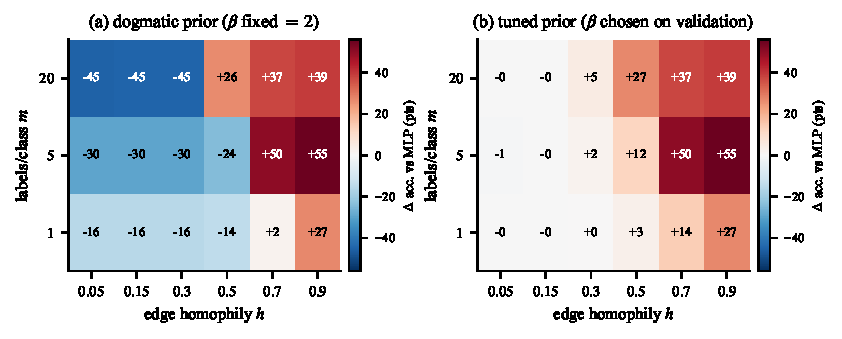
\includegraphics[width=0.95\linewidth]{fig3_sbm_heatmap.pdf}
\end{center}
\caption{Synthetic sweep: paired change in accuracy from adding the Potts MRF to the MLP,
across homophily $h$ and label budget $m$ (10 fresh graphs per cell; degree, class balance,
and feature noise held fixed). (a) Coupling fixed in advance. (b) Coupling chosen on validation
data.}
\label{fig:heatmap}
\end{figure}

\paragraph{Controls.} Three further measurements discipline the interpretation.
(i)~\emph{Rewiring:} on a degree-preserving configuration-model rewiring of Cora (edge
homophily $0.810\to0.168$), the Laplacian penalty keeps a clearly positive benefit over the GCN
($+3.24$ points at $m{=}2$, CI $[+1.82,+5.17]$, 9/10 seeds; $+2.22$ at $m{=}5$) while the
MRF's benefit vanishes ($+0.11$, CI $[-0.15,+0.74]$, and $-0.06$, CI $[-0.23,+0.15]$).
(ii)~\emph{Propagation depth:} a three-layer GCN gains $+2.91$/$+3.69$ points at $m{=}1$/$2$
with no probabilistic machinery. (iii)~\emph{Retrain-noise floor:} two GCNs differing only in
seed disagree on $16.2\%$/$14.2\%$/$6.5\%$ of test predictions at $m{=}2$/$5$/$20$, the floor
above which mechanism claims must rise. A small-validation check (selection with 5 labels/class
instead of the standard $\approx$500) preserves the main effect ($+5.64$ at $m{=}1$, 8/10;
$+7.82$ at $m{=}2$, 9/10).

\paragraph{Inference validation.} Against exact marginals (11{,}280 comparisons;
Figure~\ref{fig:fid} in the appendix): loopy BP is exact on all tree structures at every
coupling (max TV $4.8{\times}10^{-7}$, at our message tolerance); mean-field error grows
sharply with coupling everywhere ($0.19$--$0.48$ TV at $\beta{=}4$); and on the $4{\times}4$
grid at $\beta{=}1.75$, Gibbs error falls from $0.077$ to $0.007$ as kept sweeps grow from 10
to 3{,}000 while mean-field ($0.176$) and loopy BP ($0.060$) sit at fixed bias floors. At Cora
scale, mean-field and diagnostics-passing Gibbs agree to mean marginal TV $0.035$ at
$\beta\le1$; at $\beta{=}2$ Gibbs fails to mix ($\hat{R}$ up to $2.58$, ESS $4.7$ from
8{,}000 samples), so no trustworthy sampling reference exists at exactly the coupling
validation selects.

\section{Analysis}
\label{sec:analysis}

\paragraph{Why H1 reversed: an MRF amplifies evidence, it does not create it.} The selected
couplings explain the reversal mechanically. At $m{=}1$ the MLP reaches $29.2\%$ against a
$14.3\%$ chance level -- there is little label signal to propagate -- and validation
accordingly selects a weak coupling (median $\beta^\star{=}0.375$). From $m{\ge}2$ the unaries
carry real signal, validation selects the strongest coupling available, and propagation
converts feature evidence into a 19--22 point gain. Against the GCN the trend inverts for the
complementary reason: the GCN has \emph{already} propagated, so the explicit prior's marginal
value shrinks as supervision grows. The practical statement that survives is conditional: an
explicit relational prior pays in proportion to the relational information the base model has
not already extracted, provided the unary evidence is informative enough to propagate. Both
conditions failed simultaneously in the exact setting our proposal targeted (a GCN at one label
per class), which is why that experiment was the least informative one to run. Macro-F1 adds a
caution the accuracy numbers hide: at $m{=}1$ the MRF gains $+4.5$ accuracy but only $+0.9$
macro-F1, widening the accuracy--F1 gap from $7.6$ to $11.1$ points -- what little the prior
buys there, it buys on large classes while pushing small classes out of the prediction set.

\paragraph{Why the dogmatic prior fails: posterior collapse, not gradual degradation.} At
$\beta{=}2$ on the $h{=}0.05$ graph, $96.6\%$ of edges end with both endpoints predicted the
same label and accuracy falls to $16.9\%$ -- the coupling term overwhelms the unary evidence
and the MRF paints the graph one color. Interpolating each seed's zero crossing places the
break-even homophily at $h^\star=0.76\,[0.52,0.87]$, $0.57\,[0.40,0.59]$, and
$0.43\,[0.42,0.43]$ for $m{=}1,5,20$ (Figure~\ref{fig:cross}a): more supervision tolerates a
wronger prior. The tuned regime's safety is structural -- $\beta\to0$ nests the baseline, so
validation retreats when the assumption is wrong -- and it implies a methodological warning: a
study that tuned everywhere would have observed the benign panel of
Figure~\ref{fig:heatmap}(b) and concluded the prior is harmless. Harm is only observable when
the experimental design includes commitment.

\begin{figure}[t]
\begin{center}
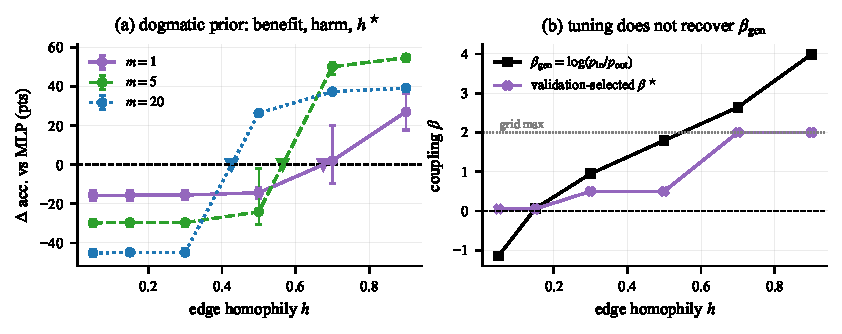
\includegraphics[width=0.95\linewidth]{fig4_crossover_beta.pdf}
\end{center}
\caption{(a) Dogmatic-regime benefit against homophily; triangles mark the median break-even
$h^\star$ per label budget. (b) Validation-selected coupling $\beta^\star$ against the
generator-implied $\beta_{\rm gen}=\log(p_{\rm in}/p_{\rm out})$: tuning moves in the right
direction but saturates at the grid maximum and cannot express the negative coupling required
below $h\approx0.15$.}
\label{fig:cross}
\end{figure}

\paragraph{A low-homophily graph is not an uninformative graph.} At $h{=}0.05$ the generator
implies a \emph{negative} coupling, $\beta_{\rm gen}=-1.15$: neighbors are informative because
they tend to differ. \textsc{Oracle-G}, using the true model with that coupling, reaches
$77.0\%$ -- above the feature-only ceiling of $73.4\%$ -- while our positive-$\beta$ prior
collapses to $15\%$. The relational evidence is valuable; the \emph{same-label} assumption has
the wrong sign, and no $\beta\ge0$ can repair a sign error (Figure~\ref{fig:cross}b). This
gives concrete, controlled form to the distinction of \citet{ma2022homophily} between
misspecified priors and uninformative graphs.

\paragraph{The Laplacian penalty is mostly generic regularization.} Proposition~1 predicted
that $\mathcal{L}_{\rm lap}$ does something a relational prior should not: penalize confidence
irrespective of the graph. The rewiring control confirms it. When label structure is destroyed
but degrees are preserved, a genuinely relational method must lose its benefit -- the MRF does
(intervals covering zero at both budgets) -- yet the Laplacian penalty retains most of its gain
on a graph whose edges carry no label information. Much of what the ``logic regularizer'' of
our proposal contributed on Cora therefore came from its confidence-penalty term, i.e.\
ordinary regularization. Two caveats bound this claim: at $m{\le}2$ a deeper GCN matches the
explicit prior's gains without probabilistic machinery, and all mechanism claims sit above the
measured retrain-noise floor.

\paragraph{Consistency is not accuracy; accuracy is not calibration.} Rule satisfaction and
edge agreement rise monotonically with $\beta$ while accuracy rises and then collapses
(appendix Figure~\ref{fig:sens}); at the collapse the model is maximally self-consistent and
minimally correct, so agreement with a symbolic rule is not a proxy for correctness. The
probability metrics repeat the caution: at $m{=}2$ the MRF improves the MLP's accuracy by 11.2
points while \emph{worsening} NLL ($1.86\to2.86$) -- confident, sometimes confidently wrong,
marginals -- and only with ample supervision does probability quality improve too
(MRF-on-GCN NLL $0.978$ vs.\ GCN $1.055$ at $m{=}20$). Calibration separates the families in
Table~\ref{tab:metrics}: the GCN variants are the worst calibrated (ECE $0.36$--$0.40$),
while the explicitly probabilistic treatments improve NLL, Brier, and ECE substantially.

\paragraph{Bias versus variance in inference.} The validation study reproduces the classical
picture \citep{murphy1999loopy} and grounds our engine choice: sampling error is variance and
shrinks with computation (Gibbs: $0.077\to0.007$), while variational error is bias and does not
(mean-field floor $0.176$). The honest negative is that at $\beta{=}2$ on Cora -- the coupling
validation selects -- Gibbs fails its own diagnostics, so the posterior there is evidently
multimodal enough to defeat a chromatic sampler at this budget, and we report that rather than
quoting numbers from unmixed chains.

\section{Limitations}

Our intervals rest on 10 seeds (30 for confirmatory cells), so coverage is approximate; on the
real datasets, seeds vary the training sample and initialization on a \emph{fixed} graph and
test set, so those intervals describe run-to-run variability rather than generalization to new
graphs -- only the synthetic experiment has graph-level replication. We study one backbone, one
pairwise prior, and the transductive setting; conclusions about other architectures or
inductive settings are not licensed. The synthetic magnitudes are conditional on $\sigma_x$,
which sets how much room the graph has to help, and at high homophily the Potts prior is
correct \emph{by construction} -- the SBM's edge log-odds have exactly the Potts form -- so the
sweep is best read as a controlled check of the measurement apparatus, with real-data results
carrying claims about real graphs. Validation selected the largest $\beta$ in our
pre-registered grid in most MRF-on-MLP cells, so the reported gains are lower bounds (an
exploratory extension appears in the appendix). Finally, two issues merit further work: the
wrong-sign failure at low homophily calls for replacing $\mathbf{1}[y_i{=}y_j]$ with a learned
$C{\times}C$ compatibility matrix estimated by EM over the unlabeled nodes -- the direction of
GMNN \citep{qu2019gmnn}, for which \textsc{Oracle-G} bounds the available gain at up to 62
points at $h{=}0.05$ -- and the mixing failure at strong coupling calls for annealed or
structured inference where chromatic Gibbs breaks down.

\section{Conclusion}

We converted an implicit architectural assumption into an explicit probabilistic model and
measured, under a pre-registered protocol with validated inference, when stating it explicitly
pays. The takeaway is a conditional statement rather than a slogan: an explicit homophily prior
helps in proportion to the relational information the base model has not already extracted and
to the quality of the evidence it can propagate -- not, as we ourselves hypothesized, in
proportion to label scarcity -- and it is dangerous only when committed to in advance, where
misspecification triggers posterior collapse below a measurable break-even homophily. The
methodological lesson travels beyond this project: a penalty described as encoding a relational
rule should lose its benefit when the relations are destroyed, and the fact that a widely used
one does not is a caution for any work that interprets regularizers as knowledge.

\subsubsection*{Reproducibility statement}

Hypotheses, comparisons, grids, seeds, and the analysis plan were version-controlled before any
experiment ran; the two post-hoc amendments are documented with rationale in the appendix.
Every number in this paper is produced by script from append-only run logs; none is transcribed
by hand. Code, the frozen protocol, raw logs, and all analysis and figure scripts accompany
this report.

\bibliography{iclr2026_conference}
\bibliographystyle{iclr2026_conference}

\appendix
\section{Appendix}

\subsection{Pre-registered comparisons}

\begin{center}
\small
\begin{tabular}{llrrl}
\toprule
& Statement & $\theta$ (pts) & 95\% CI & Outcome \\
\midrule
H1 & benefit larger at $m{=}2$ than at $m{=}20$ & $-7.07$ & $[-10.26,-3.91]$ & refuted (reversed) \\
H2a & dogmatic benefit larger at $h{=}0.9$ than $0.5$ & $+78.77$ & $[+55.53,+84.87]$ & supported \\
H2b & dogmatic prior harms at $h{=}0.05$ & $-29.72$ & $[-31.81,-28.16]$ & supported \\
\bottomrule
\end{tabular}
\end{center}
Holm-corrected two-sided Wilcoxon signed-rank tests; H1 uses 30 paired seeds, H2a/H2b use 10
freshly generated graphs each.

\subsection{Protocol amendments}

\textbf{A1.} The pre-registered Gibbs convergence gate included a maximum between-chain
difference in marginals. Implementation testing showed this measures Monte-Carlo precision at a
finite budget rather than mixing (a 12-node cycle at $\beta{=}1$ reached $\hat{R}=1.0004$ and
ESS $=5{,}540$ yet between-chain difference $0.0258$), so it would have labeled well-mixed
chains as failures. It is still computed and reported, but the pass/fail decision uses
$\hat{R}$ and ESS. Amended before any experimental result existed.

\textbf{A2.} The largest coupling in the pre-registered grid is selected in most MRF-on-MLP
cells; an extension to larger $\beta$ was run afterwards and is labeled exploratory throughout.

\subsection{Additional figures}

\begin{figure}[h]
\begin{center}
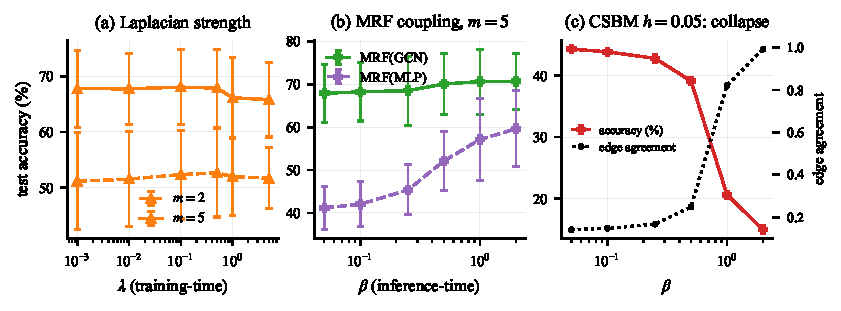
\includegraphics[width=0.95\linewidth]{fig5_sensitivity.pdf}
\end{center}
\caption{Prior strength. (a,b) Accuracy against $\lambda$ and $\beta$ on Cora; both show an
interior optimum. (c) On the misspecified synthetic graph ($h{=}0.05$), edge agreement climbs
toward 1 while accuracy falls to chance: maximal logical consistency at minimal accuracy.}
\label{fig:sens}
\end{figure}

\begin{figure}[h]
\begin{center}
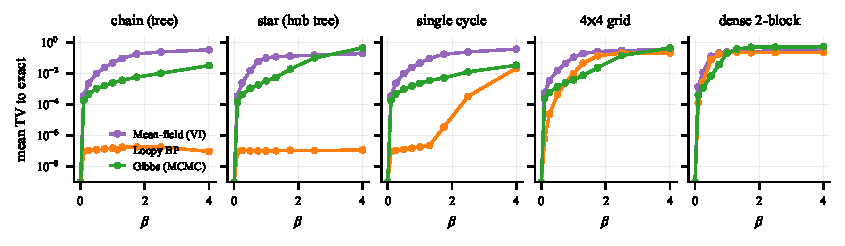
\includegraphics[width=\linewidth]{fig6_fidelity.pdf}
\end{center}
\caption{Approximate marginals against exact inference (20 random problems per point; 11{,}280
comparisons). Loopy BP is exact on trees at every coupling -- the implementation-validating
test -- while mean-field error grows steeply with $\beta$ everywhere; on loopy and dense graphs
all methods degrade at strong coupling.}
\label{fig:fid}
\end{figure}

\begin{figure}[h]
\begin{center}
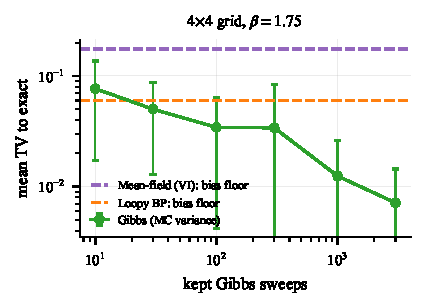
\includegraphics[width=0.5\linewidth]{fig7_bias_variance.pdf}
\end{center}
\caption{Monte-Carlo error shrinks with computation; variational bias does not. Gibbs error
against kept sweeps, with mean-field and loopy-BP floors as horizontal lines
($4{\times}4$ grid, $\beta{=}1.75$).}
\label{fig:bv}
\end{figure}

\end{document}
